\section{Mess-Server}
\label{section_Mess-Server}

Als Mess-Server wird ein BeagleBone Black von Texas Instruments eingesetzt. Dabei handelt es sich um einen kostengünstigen Einplatinencomputer mit offener Hardware. Damit ist es möglich, das BeagleBone Black auf individuelle Anforderungen anzupassen und selbst herzustellen. Auch gibt es eine große Community, die ständig die Entwicklung vorantreibt.
Er arbeitet mit einem AM335x 1GHz ARM® Cortex-A8 Prozessor, verfügt über 512MB DDR3 RAM und 4GB 8-bit eMMC internen Flash Speicher. Als Spannungsversorgung dient ein 5V 2A Netzteil.


\begin{figure}[H]
\begin{center}
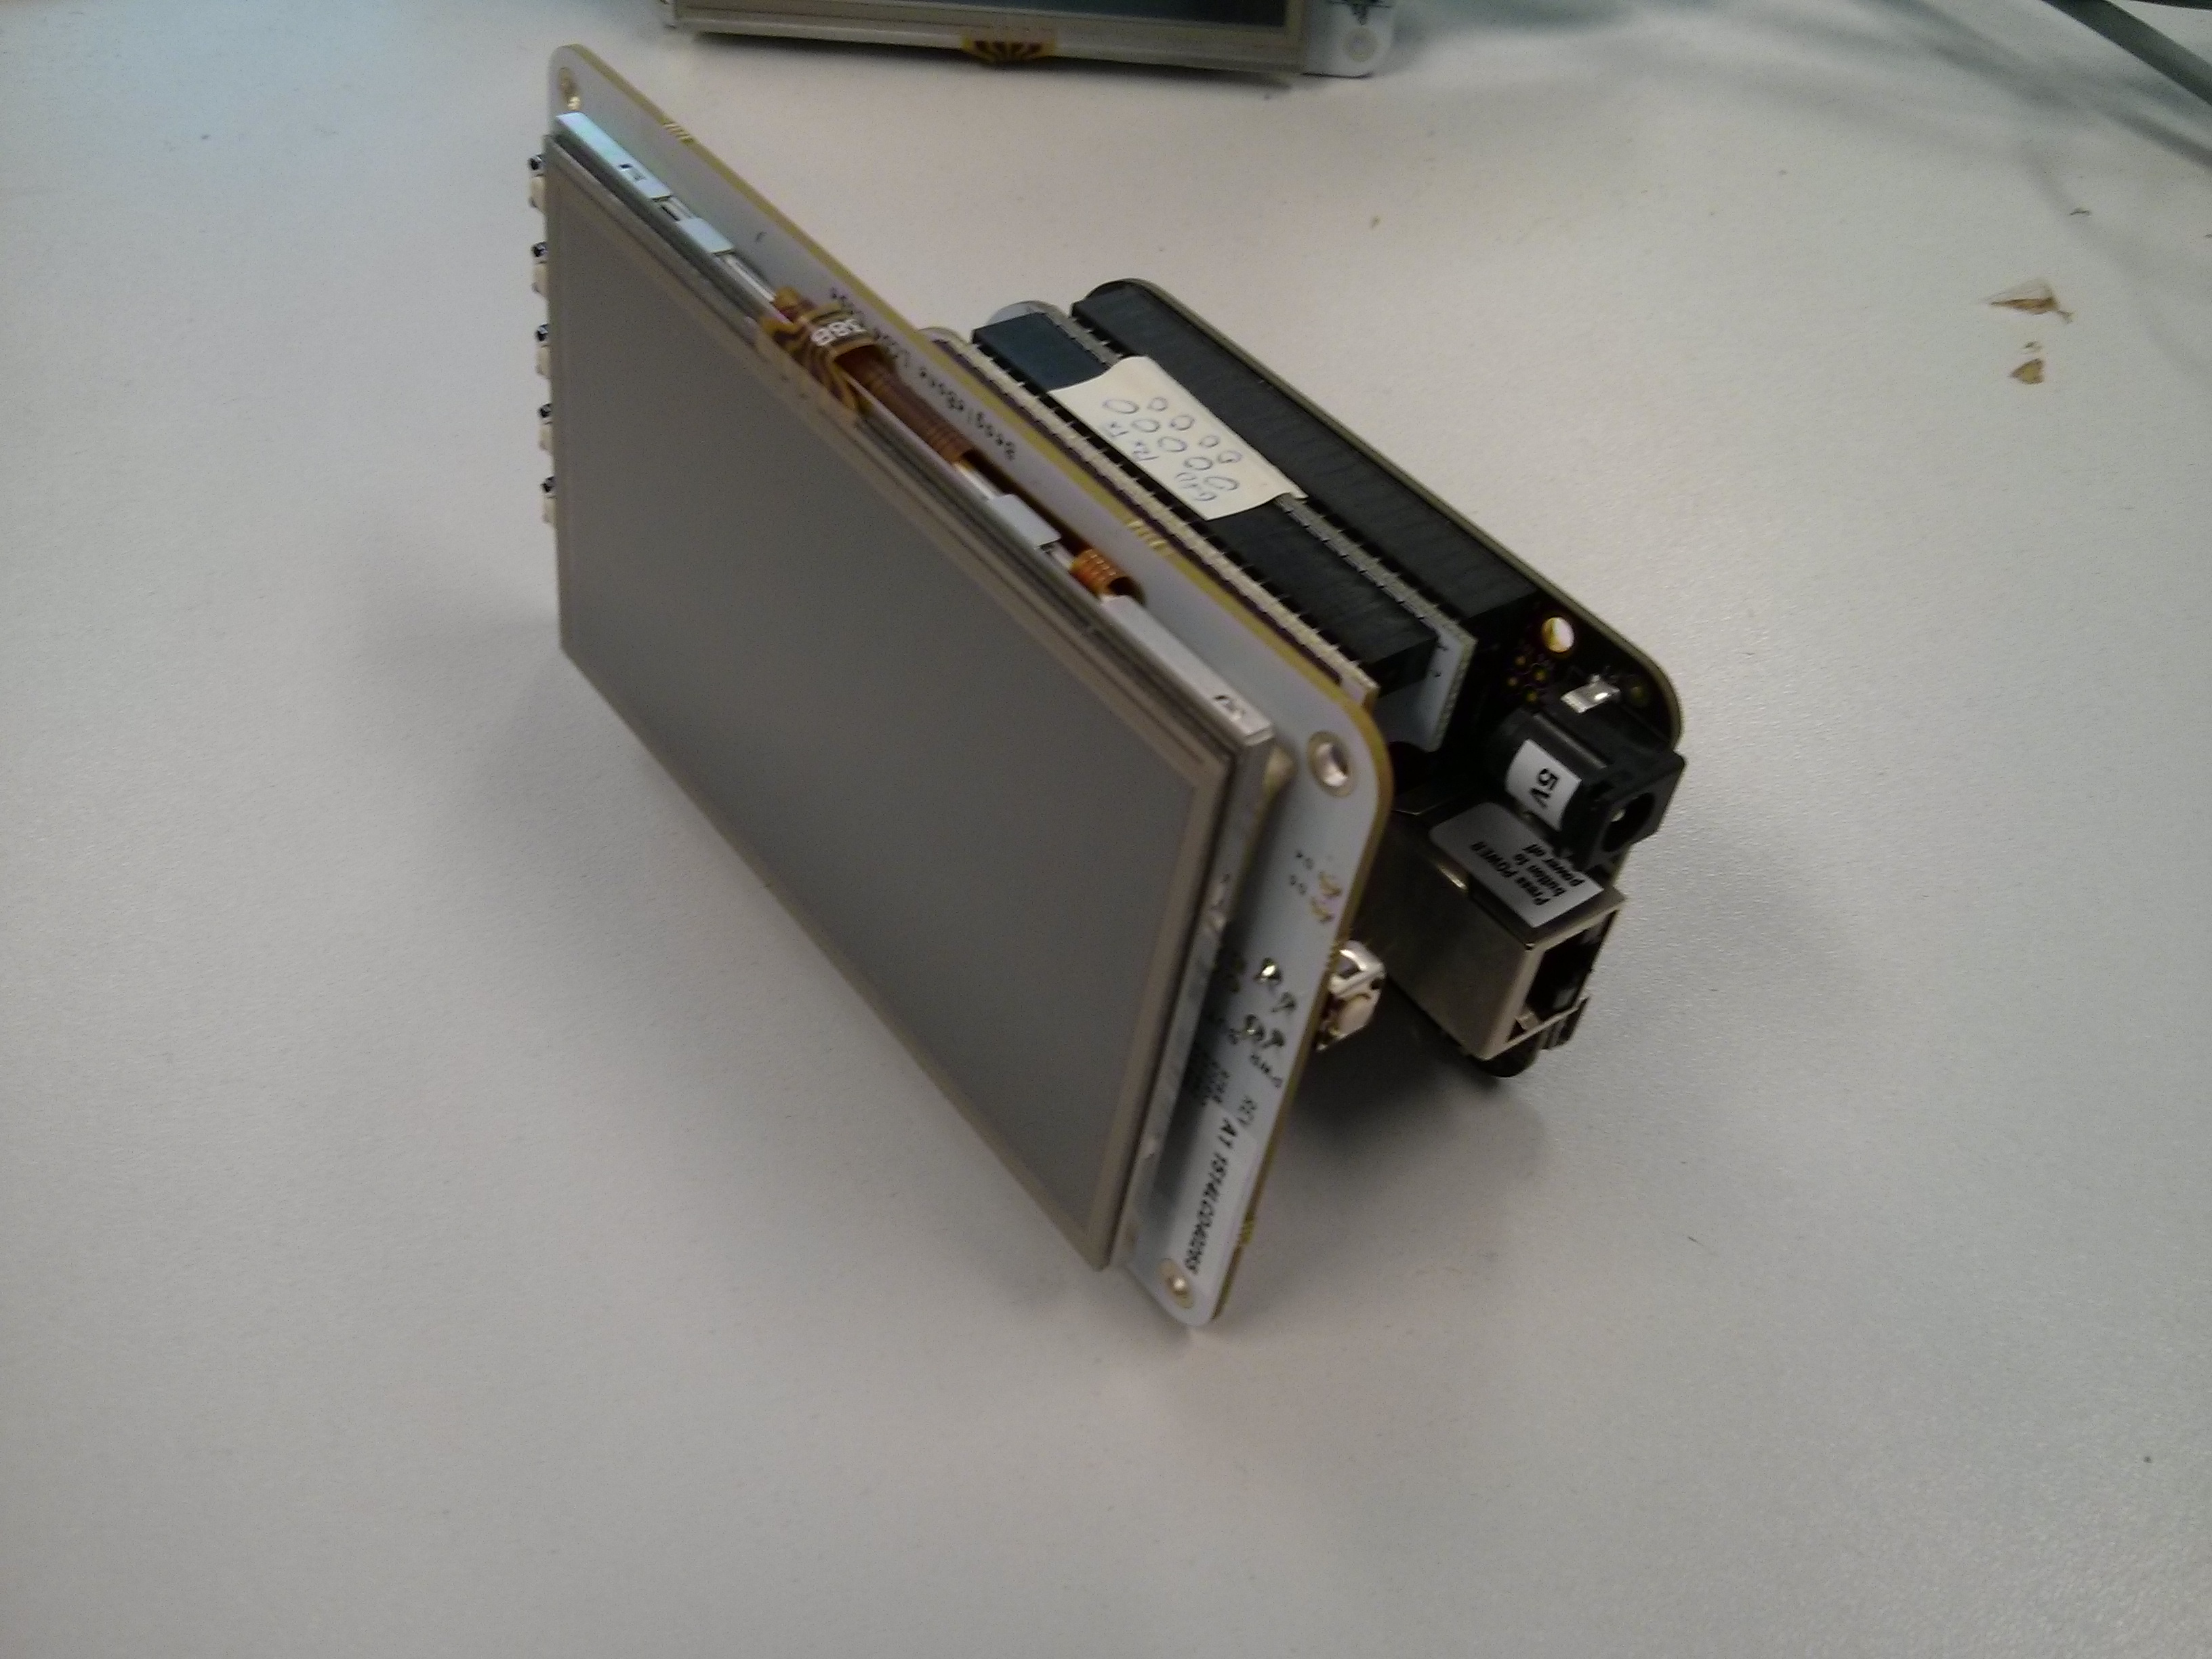
\includegraphics[width=0.8\textwidth]{img/general/BeagleBoneBlack.jpg}
\caption{BeagleBone Black}
\label{figure_Beagleboneblack}
\end{center}
\end{figure}

Trotz der Kompaktheit des BeagleBone Black, bietet er ein ausreichendes Maß an Performance. Auf ihm kommt ein Debian-GNU/Linux Betriebssystem zum Einsatz. Damit ist es möglich die umfangreichen Debian-Funktionen wie die Paketverwaltung zu nutzen. Es bietet auch den Vorteil, dass eine große Ähnlichkeit zu PC-Distributionen wie Ubuntu besteht und somit einfacher nutzbar ist(vgl. \cite{schroeder2009embedded}).\\
Außerdem sind Linux Mechanismen einfach nutzbar. So kann das \ac{UART} Interface beispielsweise wie eine normale Datei beschrieben und gelesen werden.

\subsection{Hardware}
\label{ServerHardware}

\begin{figure}[H]
\begin{center}
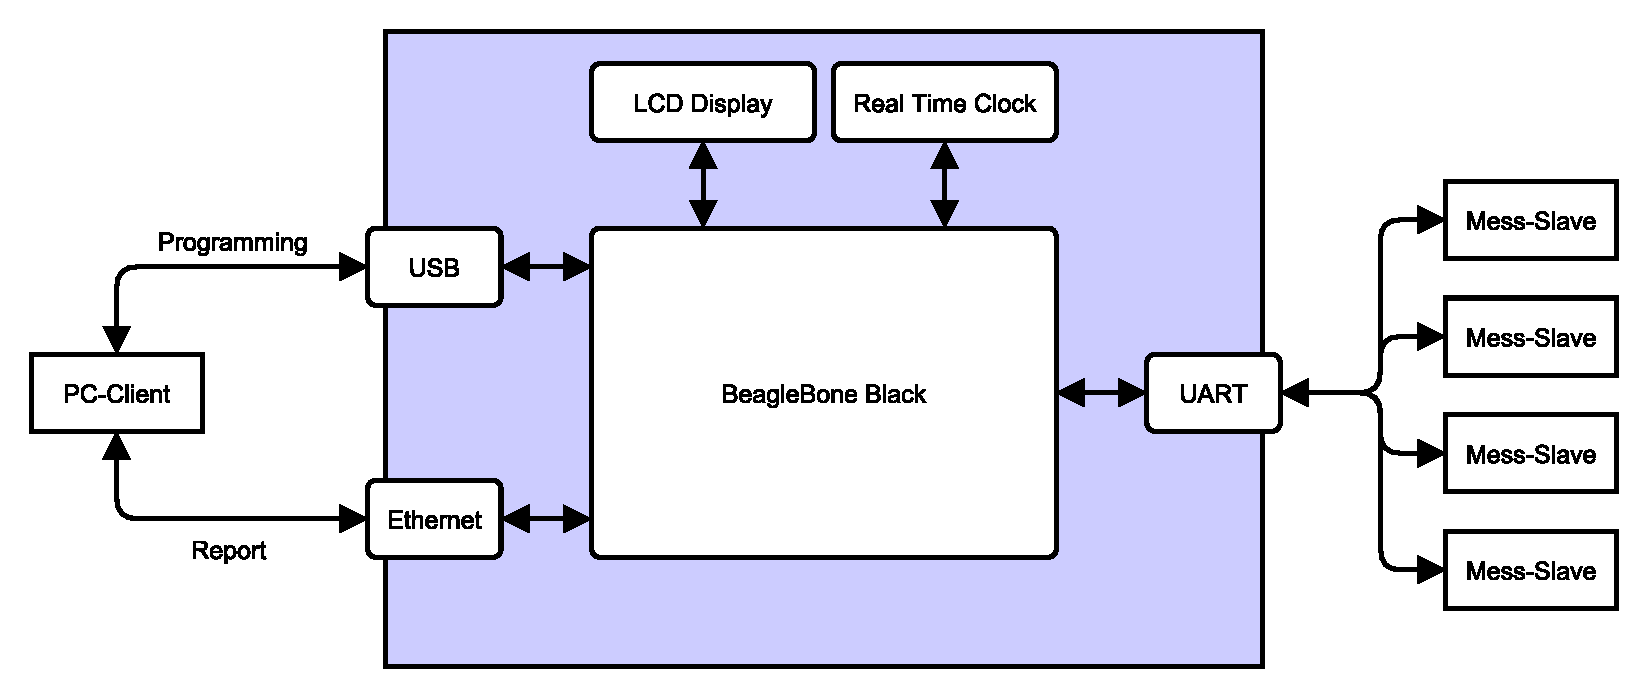
\includegraphics[width=\textwidth ]{img/general/UebersichtMaster.pdf}
\caption{Aufbau Mess-Server}
\label{figure_AufbauBleagleBone}
\end{center}
\end{figure}

Zur Kommunikation mit den Mess-Clients wird die \ac{UART} Schnittstelle des BeagleBone Black verwendet. Dafür wird ein RS232 Cape eingesetzt. Das Cape führt die seriellen Ports UART0, UART1, UART2 und UART4 auf einen 9-poligen seriellen Stecker. Es bietet die Möglichkeit zwischen den verschiedenen Ports mittels eines Jumper auf dem Cape zu wechseln.\\
Da das BeagleBone Black kein eigenes \ac{RTC} Modul besitzt, wird auch dieses durch ein Cape hinzugefügt. Es beinhaltet eine 3,3V Knopfbatterie um auch im Falle einer Stromunterbrechung die aktuelle Zeit nicht zu verlieren.\\
Um die Statusanzeige detailliert darstellen zu können, wird ein resistives LCD-Touchscreen Display eingesetzt. Es hat eine Größe von 4,3 Zoll bei einer Auflösung von 480x272 Pixeln. Dabei handelt es sich ebenso um ein Cape. Dadurch ist es möglich, das BeagleBone Black trotz den Erweiterungen kompakt zu halten. Denn die Capes sind untereinander Stapelbar.\\
Die USB Schnittstelle, welche zur Programmierung des BeagleBones verwendet wird, ist bereits vollständig einsatzbereit. Ebenso ist die Ethernet Schnittstelle, welche für den Fernzugriff auf das BeagleBone genutzt wird, bereits vollständig integriert.

\subsection{Software}
\label{ServerSoftware}
Die Programmierung der Software erfolgt in C++ unter Verwendung der Klassenbibliothek Qt (siehe Abschnitt \ref{section_Qt}).\\
Das Softwaredesign teilt sich in einen sequentiellen Teil für die Abfrage und Speicherung der Messwerte, sowie einen Event gesteuerten Teil für die \ac{GUI} und die externe Kommunikation für die Fernzugriffe. Die beiden Programmteile können unabhängig von einander agieren und kommunizieren ausschließlich über Signale und Slots (siehe \ref{QtSignaleSlots}). Durch diese Kapselung ist es möglich die beiden Programmteile durch andere Lösungen auszutauschen, welche lediglich die selben Signale und Slots unterstützen müssen.\ 

\subsubsection{Messdatenerfassung}
Der Hauptzyklus der Software ruft kontinuierlich die Messdaten von den Mess-Clients ab. Dafür wird ständig geprüft ob Messungen erforderlich sind. Dies geschieht durch den Vergleich der vergangenen Zeit zur letzten Messung und den gegebenen Parametern für die Messintervalle. In der Tabelle \ref{table_ParameterMessintervalle} finden sich diese Parameter.\\


\begin{table}[H]
\begin{center}
\begin{tabular}{|l|l|}\hline
Parameter & Beschreibung \\ \hline
duration\_int1 & Dauer der Zeit die Werte im 1.Interval aufgenommen werden in Tagen\\  \hline
duration\_int2 & Dauer der Zeit die Werte im 2.Interval aufgenommen werden in Tagen\\  \hline
interval\_1 & Abstand zwischen den Messungen im 1. Interval in Minuten\\  \hline
interval\_2 & Abstand zwischen den Messungen im 2. Interval in Minuten\\  \hline
interval\_3 & Abstand zwischen den Messungen nach dem 2. Interval in Minuten\\ \hline
\end{tabular}
\caption{Parameter der Messintervalle}
\label{table_ParameterMessintervalle}
\end{center}
\end{table}


Ob eine Messung erforderlich ist, lässt sich aus den gegebenen Parametern ableiten. So wird zuerst geprüft, welcher Zeitraum (\textit{duration\_int1-2}) derzeit zutrifft. Dazu wird die vergangene Zeit seit der ersten Messung mit dem Zeitraum abgeglichen. Sollten noch keine Ergebnisse vorhanden sein, ergibt dies die Erforderlichkeit einer Messung. Wenn der passende Zeitraum ausgemacht ist, wird das dazugehörige Intervall zwischen den einzelnen Messungen (\textit{interval\_1-3}) ausgemacht. Dann wird geprüft, ob die vergangene Zeit seit der letzten Messung größer als dieses Intervall ist.\ 

Anschließend wird geprüft ob der Mess-Client verfügbar ist. Dazu wird eine Namensanfrage über die RS232 Schnittstelle verschickt.\\
Bei einer positiven Antwort wird dann eine Messung durchgeführt. Dabei werden alle \acp{ADC} der 64 möglichen \acp{DUT} mittels \textit{ADC-Value}-Befehls (siehe Tabelle \ref{table_Commands}) ausgelesen. Sobald alle 64 Werte erfolgreich ermittelt wurden, werden sie in der Datenbank abgelegt.
 
 
\subsubsection{Benutzeroberfläche}
Zur Statusüberwachnung verfügt das BeagleBone über eine \ac{GUI}. Sie bietet einen einfachen Überblick über die aktuellen Vorgänge und soll auf einen Blick den Status des Mess-Servers wiedergeben. 


\subsubsection{RS232 Kommunikation}
Die RS232 Schnittstelle wird ausschließlich zur Kommunikation mit den Mess-Clients verwendet. Um die Erfolgschancen der Anfragen zu erhöhen, werden Fehlschläge erkannt und durch den Versuch des erneuten Sendens minimiert. Zwischen jedem Sendeversuch befindet sich eine kurze Verzögerung.
 
\subsubsection{Datenbankanbindung}

Auf dem Beaglebone kommt ein MySQL Server als Datenbanksystem zum Einsatz (siehe Abschnitt \ref{section_Datenbank}). Der Zugriff erfolgt mittels der von Qt bereitgestellten QtSQL Klassen.

\subsubsection{Ethernet Kommunikation}

Um auf Netzwerkanfragen reagieren zu können, ist sowohl ein UDP-Server für Broadcast-Nachrichten als auch ein TCP-Server für die direkte Kommunikation realisiert.\\
Der UDP-Server dient dabei zur dynamischen Erkennung im Netzwerk. Dabei antwortet der Mess-Server auf Broadcast-Nachrichten mit seiner IP-Adresse und seinem Namen. Dies ermöglicht die einfache Eingliederung der Mess-Server in ein Netzwerk.

